\subsection{Organização do projeto}
Tal como o \textit{backend}, o modelo a seguir no \textit{frontend} foi o \textit{\acrshort{mvc}}. 

Como recomendado de boas práticas de código limpo da \textit{framework}, as cores do tema da aplicação foram colocadas num ficheiro separado para garantir a fácil troca do tema da aplicação. Outras aplicações de boas práticas de código limpo foram, sempre que possível, particionar o código das páginas em vários \textit{widgets}, para deste modo, facilitar a navegação e também, a criação de \textit{widgets} reutilizáveis que evitam a repetição de código e agilizam o desenvolvimento. Por fim, a estrutura do projeto foi organizada da seguinte forma:
\begin{figure}[htb]
 \centering
 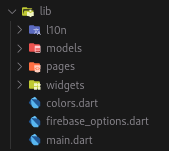
\includegraphics[width=0.35\textwidth]{images/implementacao/frontend/organizacao_projeto.png}
 \caption{Organização do projeto}
 \label{fig:69}
\end{figure}

\begin{itemize}
 \item \textbf{l10n} - Traduções da aplicação;
 \item \textbf{models} - Modelos de classes como \textit{handlers, helpers, providers}, entre outros;
 \item \textbf{pages} - Páginas da aplicação;
 \item \textbf{widgets} - \textit{Widgets} referentes às páginas;
\end{itemize}
\vspace{50mm}

